\documentclass[10pt]{beamer}

\usepackage{natbib}

\usetheme[progressbar=frametitle]{metropolis}
\usepackage{appendixnumberbeamer}

\usepackage{booktabs}
\usepackage[scale=2]{ccicons}

\usepackage{pgfplots}
\usepgfplotslibrary{dateplot}

\usepackage{xspace}
\newcommand{\themename}{\textbf{\textsc{metropolis}}\xspace}

\usepackage{amsmath, bm}
\usepackage[ruled,vlined]{algorithm2e}

\title{Approximate Bayesian Computation}
\subtitle{}
% \date{\today}
\date{}
\author{Davi Barreira}
\institute{FGV - Escola de Matemática Aplicada}
% \titlegraphic{\hfill\includegraphics[height=1.5cm]{logo.pdf}}

\begin{document}

\maketitle

% \begin{frame}{Table of contents}
%   \setbeamertemplate{section in toc}[sections numbered]
%   \tableofcontents%[hideallsubsections]
% \end{frame}

\section[Introduction]{Introduction}
\begin{frame}[fragile]{Objective}

  The objective of this presentation is to give an overview of
  the Approximate Bayesian Computation (ABC) algorithm through the
  replication of the
  paper \textbf{Approximate Bayesian computational methods} by
  \cite{Marin2012}.

  The paper talks about different variants of ABC by estimating the
  posterior of Moving Average models.

\end{frame}

\begin{frame}[fragile]{Motivation}

  ABC methods are known as likelihood-free techniques, thus are
  a useful approach in problems that the likelihood is intractable, e.g., likelihood not available in
  closed form, or likelihood too expensive to calculate.
  \begin{itemize}
    \item Coalecent models in population genetics \citep{Tavare505};
    \item Species dynamics \citep{Jabot2016};
    \item Real-world model of HIV transmission \citep{McKinley2018}.
  \end{itemize}

\end{frame}

\begin{frame}[fragile]{Motivation}

  In some settings where we have latent variables, the likelihood is
  expressed as:
  $$\ell(\bm\theta \mid \bm y) =
  \bm\int \ell^*(\bm\theta \mid \bm y, \bm u) d\bm u$$

  Hence, $\bm y$ is observed and $\bm u$ is latent and $\bm\theta$
  is the parameter of interest.

\end{frame}

\begin{frame}[fragile]{Original Algorithm}

  \citet{Rubin1984} described the ABC algorithm as a thought experiment
  to explain how to sample from a posterior distribution.
  \citet{Tavare505} is usually considered the paper responsible for the
  proposing ABC for infering the posterior distribution.

  \vspace{1cm}

\begin{algorithm}[H]
\SetAlgoLined
\For{i=1 to N}{
 \Repeat{$\bm y = \bm z$}{
    Sample $\bm\theta' \sim \pi(\cdot)$

    Generate $\bm z \sim p(\cdot \mid \bm\theta')$
 }
  
}
 \caption{Original ABC method}
\end{algorithm}


\end{frame}

\begin{frame}[fragile]{Original Algorithm}

  Below we have an schematic drawing with an example of
  the ABC method for Beta/Binomial model.
    \begin{figure}[H]
        \centering
        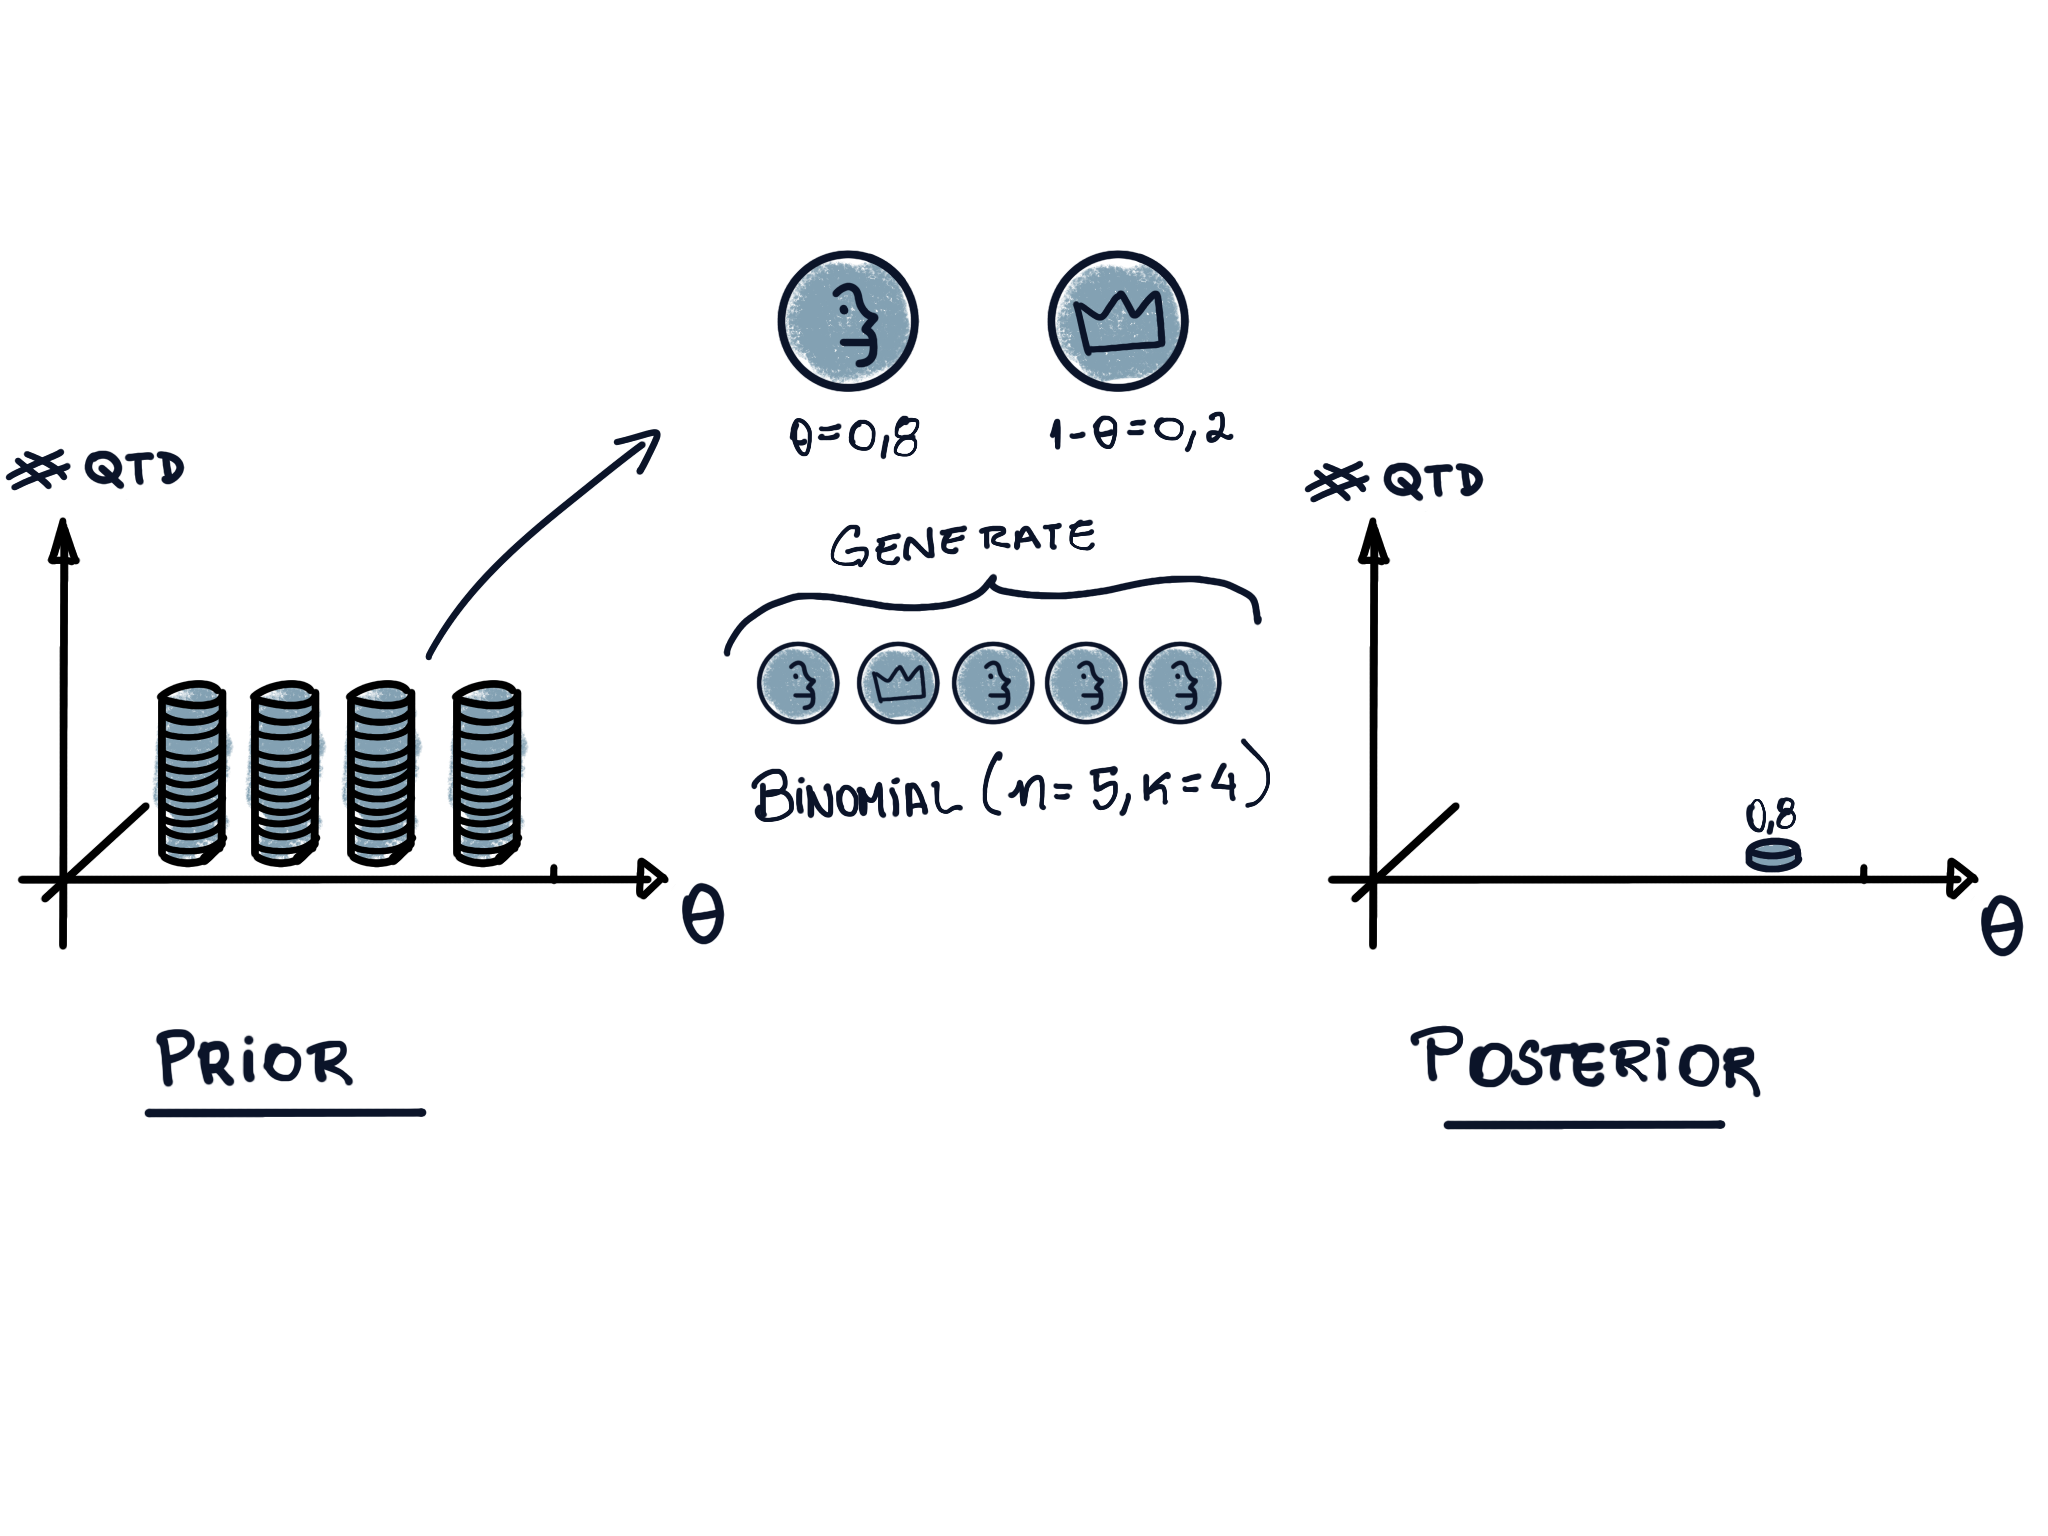
\includegraphics[width=10cm]{images/Vis-ABC.png}
        \caption{Schematic drawing of ABC method for Beta/Binomial
        model
        }
    \end{figure}

\end{frame}

\begin{frame}[fragile]{Original Algorithm}

  \citet{Pritchard1999} extended the original algorithm to the case
  of continuos sample spaces.

  \vspace{0.3cm}

\begin{algorithm}[H]
\SetAlgoLined
\For{i=1 to N}{
 \Repeat{$\rho[\eta(\bm y) , \eta (\bm z)] \leq \epsilon$}{
    Sample $\bm\theta' \sim \pi(\cdot)$

    Generate $\bm z \sim p(\cdot \mid \bm\theta')$
 }
  
}
 \caption{ABC method for discrete and continuous distributions}
\end{algorithm}
\begin{itemize}
  \item[--] $\eta$: function defining a statistic (e.g. the mean),
  \item[--] $\rho$: a distance function,
  \item[--] $\epsilon$: acceptance tolerance.
\end{itemize}

\end{frame}

% \appendix

\begin{frame}[allowframebreaks]{References}

% \renewcommand{\bibsection}{\section{}}
  \renewcommand{\section}[2]{}%
  \bibliography{abc}
  % \bibliographystyle{plainnat}
  % \bibliographystyle{plain}
  % \bibliographystyle{abbrv}
  \bibliographystyle{apa}

\end{frame}

\end{document}
